\section{Experimental Results}
\label{sec:result}
%%% First Steps and Evaluation (10 points):
%Were the first steps described in the project proposal completed?  Are
%there nontrivial preliminary results in terms of system performance or
%data collection (if data collection is a significant part of the
%project)?  Is the interpretation of these results careful and correct?  Is
%there an assessment of where the project stands?  Are next steps clear,
%including any course corrections based on preliminary results?

We have successfully completed the first steps in the proposal.
We implemented a deep learning neural network using Matlab and then
switched to python because python has a nice deep learning library,
Theano.

Using the python library Theano, we added noise to Logistic Regression
model and Multi-layer Logistic Regression model.
As a first step, we have only added noise from binomial and gaussian
distribution. Adding noise from other distributions will be studied in
the second half of the project.

\subsection{Logistic Regression}
In Logistic Regression Model, we added noise to the learning rate.
To be more specific, the weight is updated as

\begin{center}
$W_{new} = W_{old} - learningRateBinomial * \bigtriangledown_{W}$
$W_{new} = W_{old} - learningRateGaussian * \bigtriangledown_{W}$
\end{center}

where $learningRateBinomial$ is a matrix with entries from a binomial
distribution $Bin(1,0.5)$ and $learningRateGaussin$ is a matrix with entries
from a gaussian distribution $\mathcal{N}(0.26,0.13)$.

Our experiments show that adding noise to learning rate can indeed
improve accuracy of the model.

\begin{figure}[h]
\centering
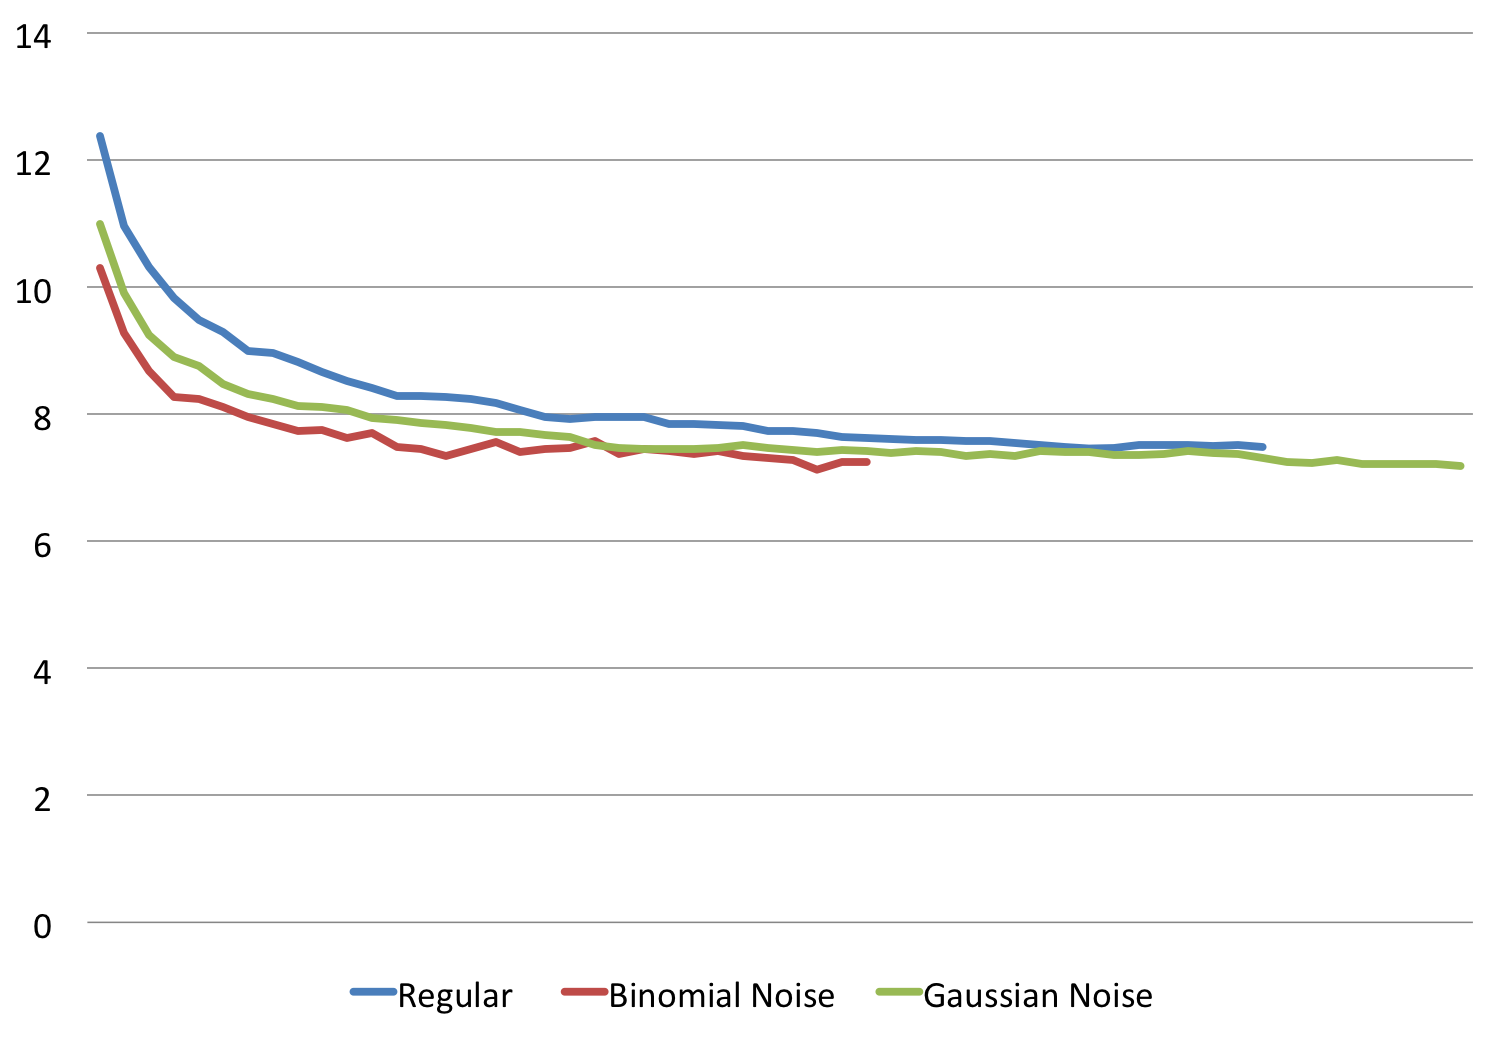
\includegraphics[width=215pt]{figs/logistic_sgd_all.png}
\caption{Logistic Regression with Noise}
\label{fig:logistic-sgd}
\end{figure}

Figure~\ref{fig:logistic-sgd} shows the accuracy of three models.
The blue line shows the test error rate of a regular Logistic Regression
Model.  The green line shows the test error rate of a Logistic Regression
Model with gaussian noise added to the learning rate.  The red line shows
the test error rate of a Logistic Regression Model with binomial noise
added the learning rate.  The models with noise outperform the regular
model through the whole training process.  We also observe that the red
line is less smooth than the green line.  This behavior is expected since
if the learning rate is from a binomial distribution, it is possible that
during the gradient descent we will step back several times.

In general, the model with binomial noise converges faster than the model
with gaussian noise, but eventually they have the same best test error
rate.

The result of this experiment is very interesting since we did not
expect that adding noise to learning rate would improve the accuracy
of the model. We will study the theoretical reason behind this improvement
of accuracy later in the project.

\subsection{Multi-layer Logistic Regression}
In Multi-layer Logistic Regression Model, we applied a random $0/1$ mask to
weights in the model to simulate DropConnect and Dropout
(See Related Works for more details about DropConnect and Dropout).
In our experiment, we tried two different values of $p$, where $p$ is
the probability of having $1$ in the mask.

\begin{figure}[h]
\centering
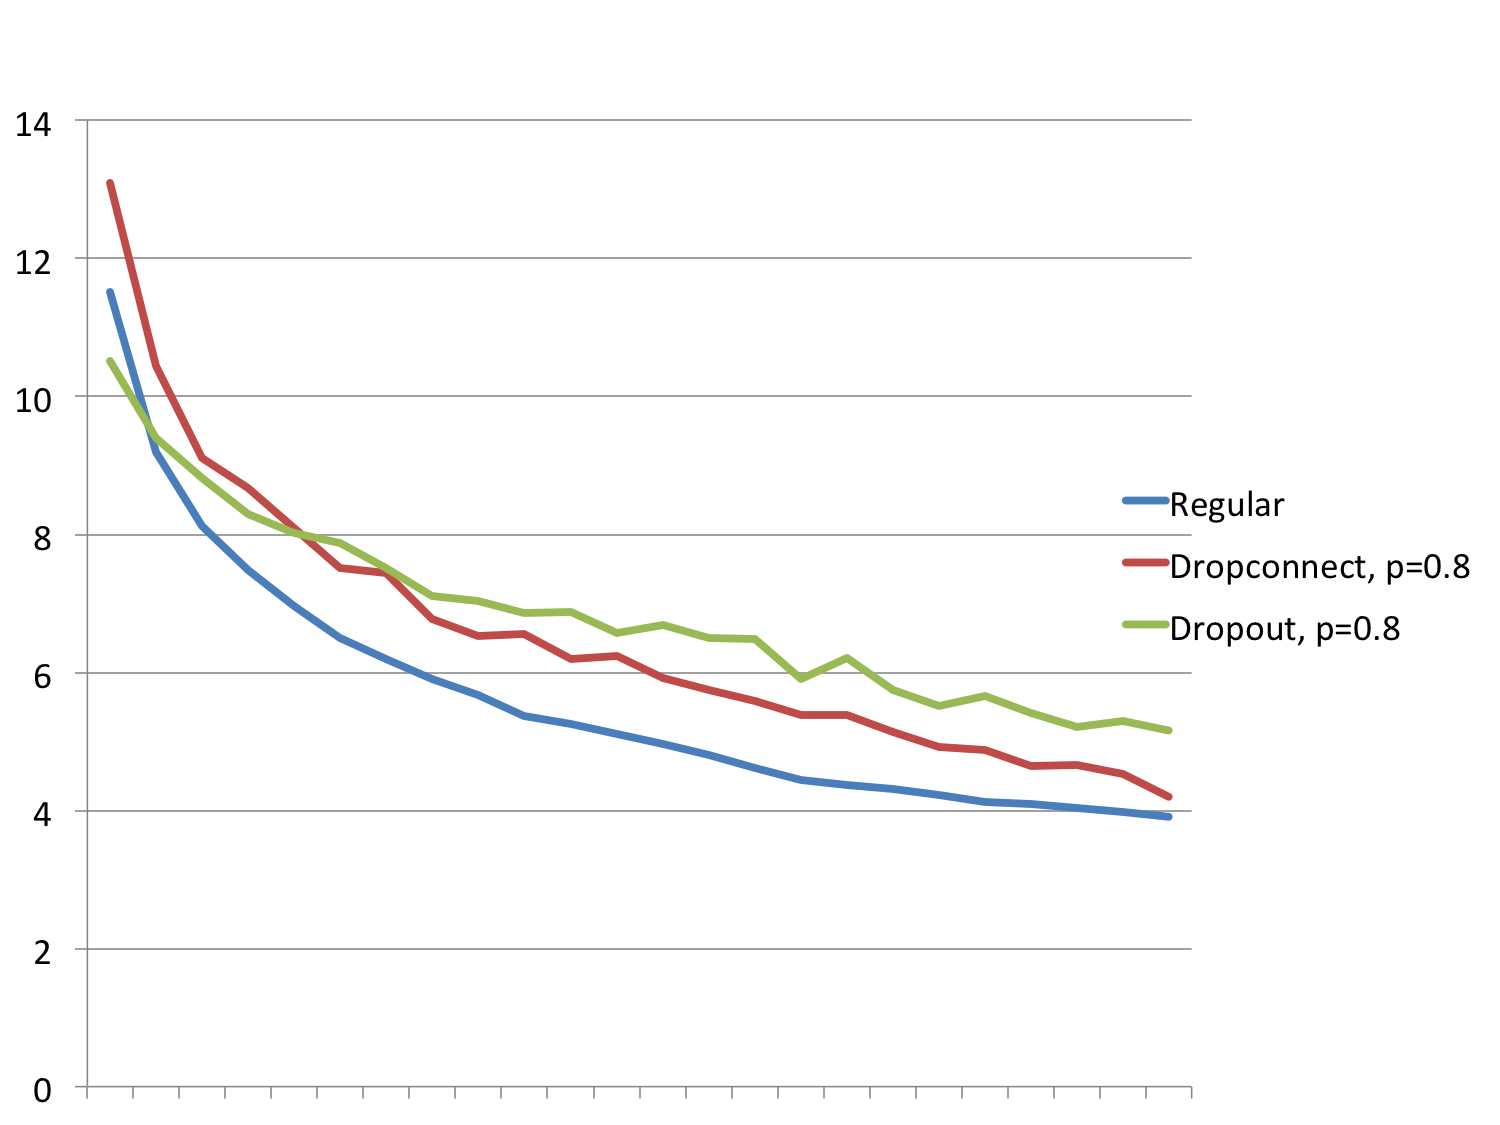
\includegraphics[width=215pt]{figs/mlp_psmall.png}
\caption{Multi-layer Logistic Regression with Noise, $p=0.8$}
\label{fig:mlp-noise-psmall}
\end{figure}

As showed in~\ref{fig:mlp-noise-psmall}, accuracy of the model was not
improved by applying a random $0/1$ mask with probability $p=0.8$.
We conjecture that this is because the number of hidden unites in the
model. In our experiment, we only have $50$ hidden units. Hence $p=0.8$ is
too small; we need to keep more weights in the model.

Based on the previous observation, we then applied a random $0/1$ mask
with $p=0.99$ to the Multi-layer Logistic Regression Model. The result
shows that the accuracy of the model is improved.

\begin{figure}[h]
\centering
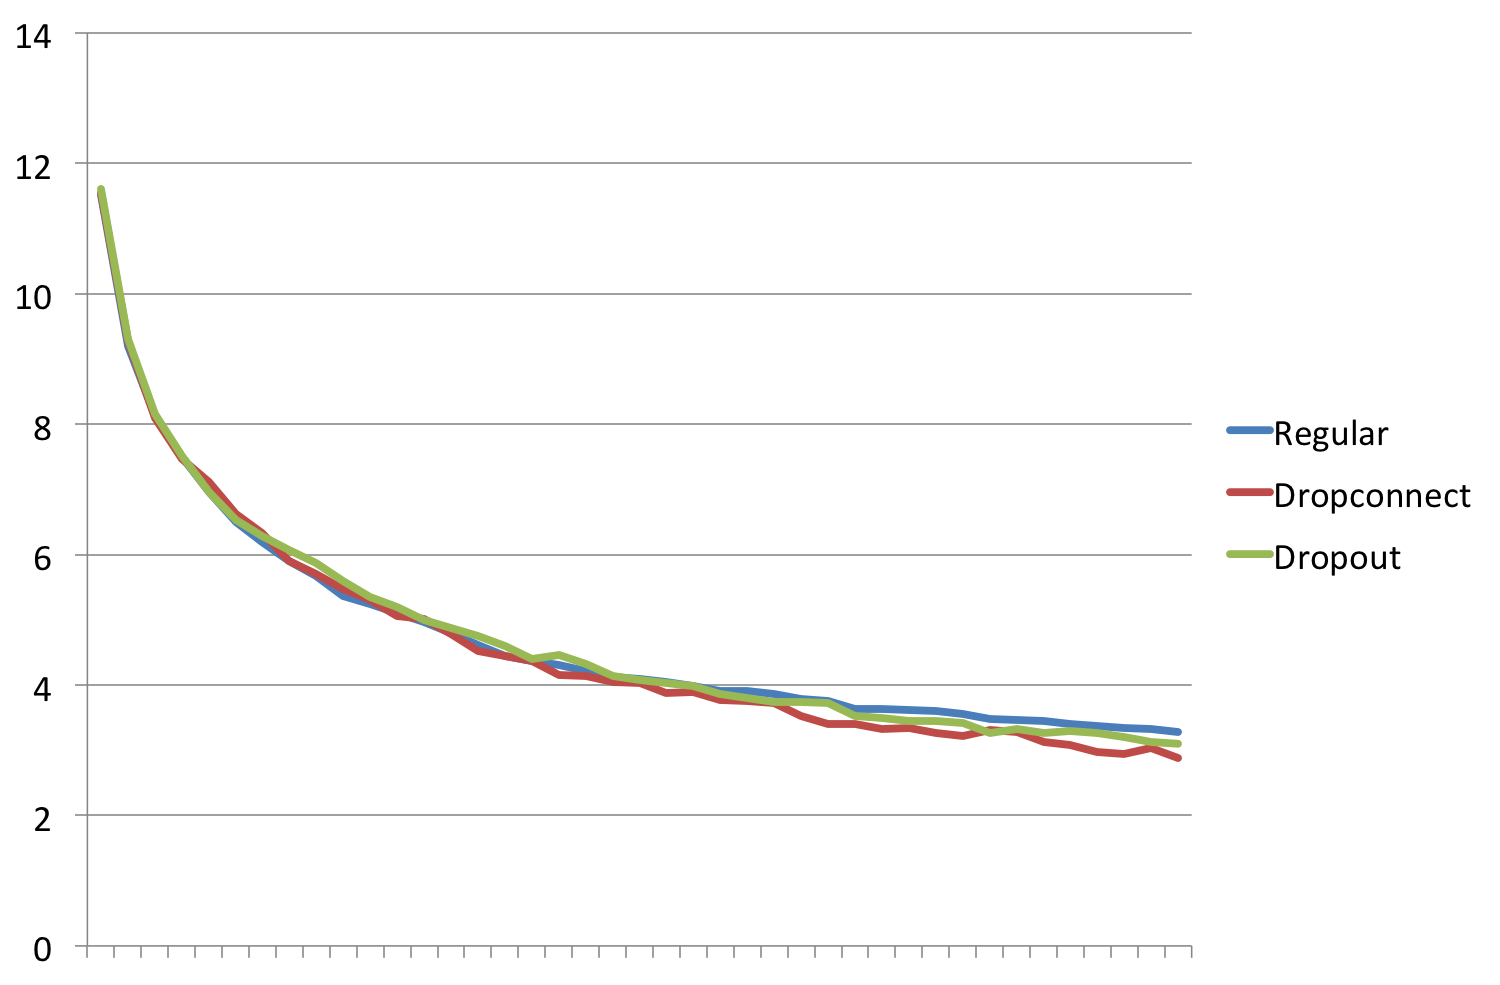
\includegraphics[width=215pt]{figs/mlp_pbig.png}
\caption{Multi-layer Logistic Regression with Noise, $p=0.99$}
\label{fig:mlp-noise-pbig}
\end{figure}

Figure~\ref{fig:mlp-noise-pbig} shows the test error rate of the
applying a random mask with $p=0.99$ to the Multi-layer Logistic
Regression Model.
The blue line shows the test error rate of a regular Multi-layer Logistic
Regression model without mask.
The red line show the test error rate of a Multi-layer Logistic Regression
Model with a random $0/1$ mask applied between input layer and hidden
layer, which simulates DropConnect.
The green line shows the test error rate of a Multi-layer Logistic
Regression model with a random $0/1$ mask applied between hidden layer and
output layer, which simulates Dropout.

The test error rate of these three models are competitive with each other.
However, the test error rate of models with noise decrease faster than
then regular one. This result is very interesting because it demonstrates
that adding noise to the model can indeed improve its accuracy.
Based on the result of this experiment, we are more interested in how to
find the optimal $p$ for a model with $n_hidden$ hidden units. We want to
know whether the optimal $p$ value depends on $n_hidden$ or not.

We are currently working on adding noise to Convolutional Multi-layer
Logistic Regression Models. Our experiment will include adding noise to
both the feature mapping part and training part.

As for next steps, we will keep adding noise from different
distributions to different neural network models.
Moreover, we want to understand why and how the noise will improve the
accuracy of the model. We also want to study how to find the optimal
noise for different models.

